\documentclass[11pt]{article}
\usepackage[margin=1in]{geometry}
\usepackage{graphicx}
\usepackage{booktabs}
\usepackage{hyperref}
\hypersetup{colorlinks=true,linkcolor=blue,urlcolor=blue}
\title{Episode End-State Classification Report}
\author{TP2 SPY Call Pipeline}
\date{June 2026}
\begin{document}
\maketitle

\section*{Purpose}
Episode tracking converts repeated daily TP2 violation rows into one economic
event. End-state classification then asks what happened on the next trading
session after the episode stopped violating.

\section*{End-State Definitions}
\begin{itemize}
  \item \textbf{true reversion}: all four legs are observable, pass clean quote
  quality, and the TP2 inequality no longer violates.
  \item \textbf{still violation or reappeared}: the same pair still violates on
  the next observable session.
  \item \textbf{liquidity filter failure}: the legs are present but do not pass
  the active tradability filter.
  \item \textbf{left/right leg missing or expired}: at least one required leg is
  no longer available, so the pair cannot be treated as a clean reversion.
  \item \textbf{sample ended}: there is no future session in the available data.
\end{itemize}

\section*{Full-Sample Counts}
\begin{center}
\begin{tabular}{lrr}
\toprule
End state & Episodes & Share \\
\midrule
true reversion & 1,059,366 & 50.64\% \\
right leg missing or expired & 536,657 & 25.65\% \\
liquidity filter failure & 315,233 & 15.07\% \\
left leg expired or missing & 151,072 & 7.22\% \\
still violation or reappeared & 28,180 & 1.35\% \\
sample ended & 1,315 & 0.06\% \\
\bottomrule
\end{tabular}
\end{center}

\begin{figure}[h]
\centering
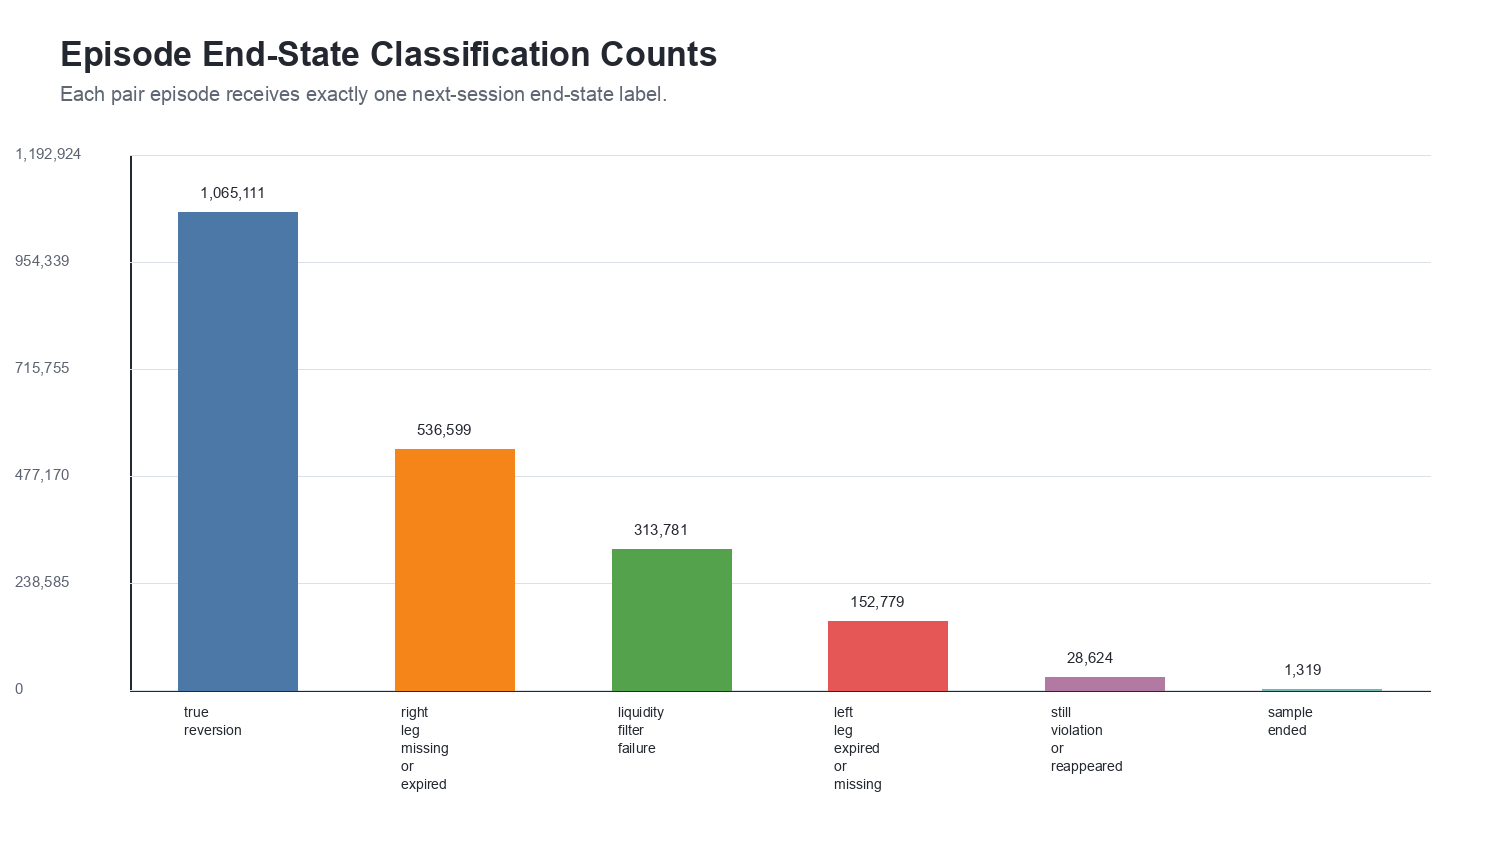
\includegraphics[width=\linewidth]{figures/episode_end_state_counts.png}
\caption{Episode end-state counts.}
\end{figure}

\begin{figure}[h]
\centering
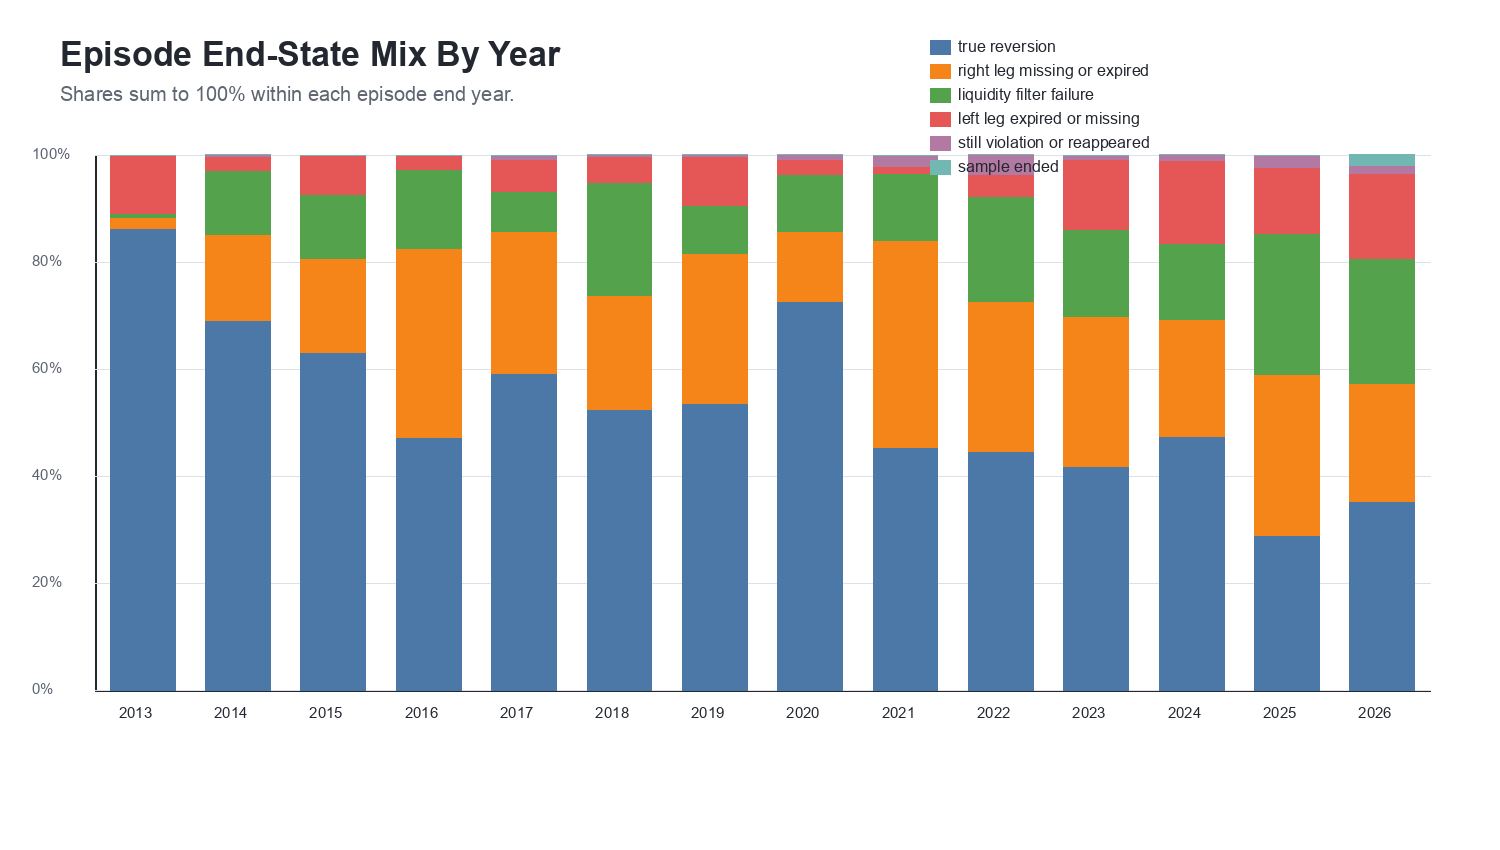
\includegraphics[width=\linewidth]{figures/episode_end_state_mix_by_year.png}
\caption{End-state composition by year.}
\end{figure}

\section*{Interpretation}
The majority of observable stopped episodes are true reversions, but missing,
expired, and liquidity-failed cases are substantial. The pipeline therefore
does not silently treat disappearance as reversion. This is important for both
paper credibility and leakage-safe ML labels.

\end{document}
